\providecommand{\rasd}{..}
\documentclass[../RASD.tex]{subfiles}

\begin{document}
    \chapter{Overall description}\label{ch:overall-description}
    \section{Product perspective}\label{sec:product-perspective}
    In the previous section, the scope of the application was delimited and explained in a shallow way, but at this point it is useful to include further details on the shared phenomena and a domain model as a visual representation of the system.

    \begin{figure}[H]
        \centering
        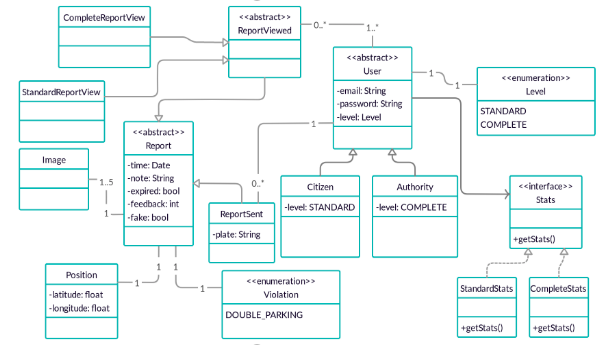
\includegraphics[scale = 1.1]{assets/domainModel.png}\\[1.6 cm]
        \caption[Domain Model \textit{Class Diagram}]{Domain Model \textit{Class Diagram}}
    \end{figure}
    Generic violation report:

    To understand the main events happening in the system, it is useful to use statechart diagrams (described in the figure below). At the beginning each report (i.e. when a user uploads an image) is considered as unprocessed. While the constraints are checked (there must be at least one photo, the type of violation, the position, if it’s a car violation the license plate is mandatory too as a picture), the report is on a pending state and can become either rejected or approved.

    Then SafeStreets checks if the report is already present in the database but the final choice is done by the user: user can choice to add or not the new report.

    In the end, it’s considered completed and the user is notified with the outcome. If it’s been approved, the report is kept in the database.
    \begin{figure}[H]
        \centering
        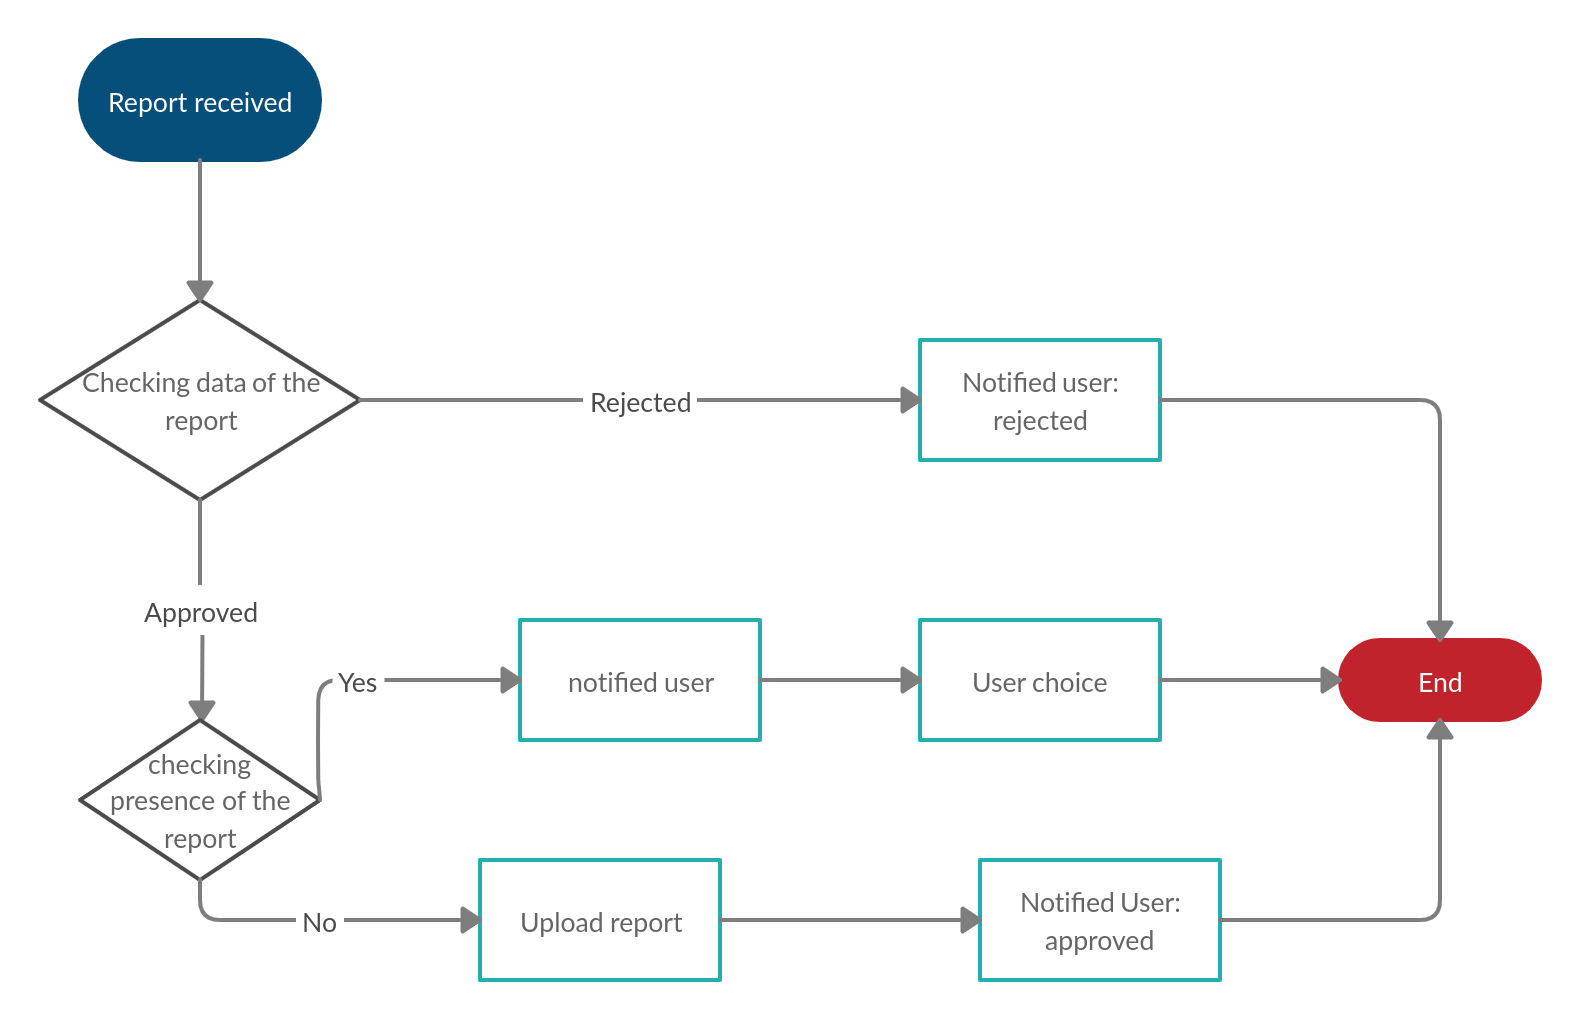
\includegraphics[scale = 0.3]{assets/newReportV2.png}\\[1.6 cm]
        \caption[ New report \textit{State Chart Diagram}]{ New report \textit{State Chart Diagram}}
    \end{figure}

    Query to database:

    In case there is a query for get information about one selected violation, it can be made by a citizen or by an authority and this establishes different results showed by the system: in the former case SafeStreets returns information and photos about selected violation but doesn’t show photos about license plate for privacy reason (system must guarantee anonymity) instead in the latter case SafeStreets returns all the photos and other information about violation so authority can use them to generate traffic tickets.

    \begin{figure}[H]
        \centering
        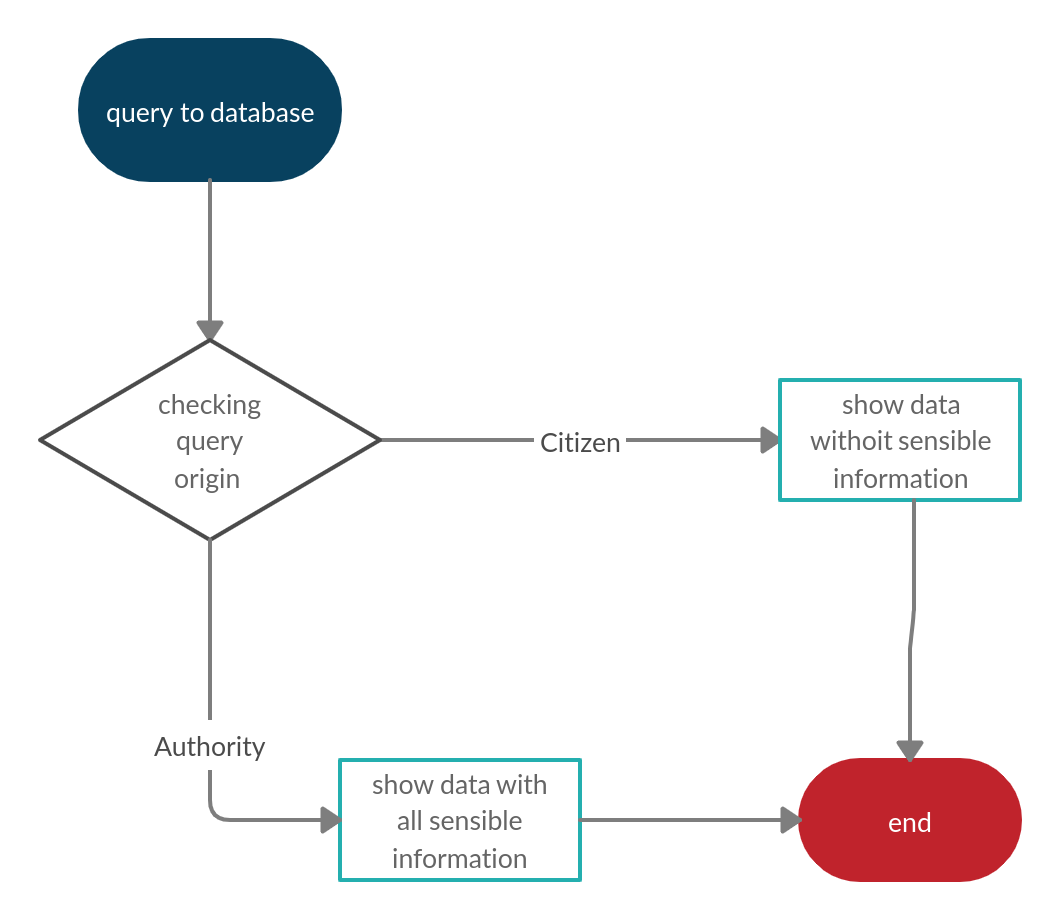
\includegraphics[scale = 0.3]{assets/queryDbV1.png}\\[1.6 cm]
        \caption[ Query to database \textit{State Chart Diagram}]{ Query to database \textit{State Chart Diagram}}
    \end{figure}


    Build statistics:

    When one authority uses a violation taken from SafeStreets and then he generates a traffic ticket form it, he marks the violation as fined.

    The system periodically builds statistics analyzing the usage of violation by the authority (marked fined or not ) to show the effectiveness of the application.

    Furthermore, SafeStreets can access to a db of the authority in which they upload data on incidents so

    it can also analyzes, querying the databases, the different type of the violation and incidents and the vehicles involved. These information are both used to build statistics and to find unsafe area(also using data about accidents), in the last case system provide a suggestion for the problem.

    \begin{figure}[H]
        \centering
        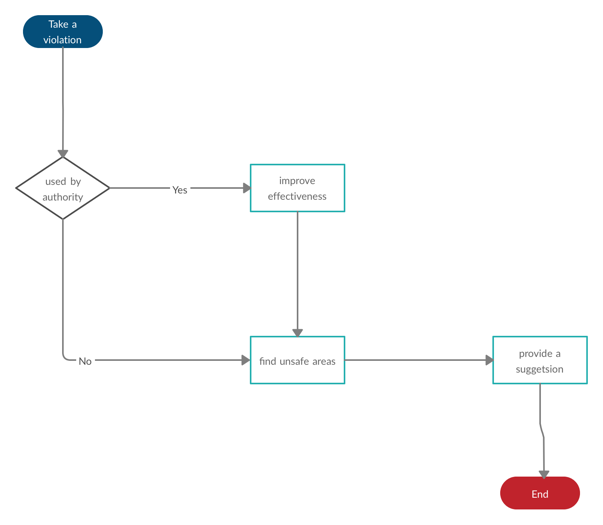
\includegraphics[scale = 3]{assets/buildStatistics.png}\\[1.6 cm]
        \caption[ Build statistics \textit{State Chart Diagram}]{ Build statistics \textit{State Chart Diagram}}
    \end{figure}

    \section{Product functions}\label{sec:product-functions}
    In the following we will present the main aspects and functions of the system, to put in evidence the most important requirements that will be formalized in chapter 3.
    \subsection{Citizens functions}\label{subsec:citizen-functions}
    A person can register himself to the SafeStreets system by providing a valid email address and a password. No other data will be mandatorily required, but the user will be allowed to set a residential location to personalize the user interface.

    Every registered user that see a traffic violation can report it throw SafeStreets: to do that, he must upload at least one photo of the infringement and provide some information about it. The pictures can be only taken by a specific tool of the application that won't allow to modify the photos; this restriction is applicate to not let people to upload pictures that could have been modified to accuse someone extraneous to the burglary. The user will have to add to the images the position (that will be possible to be taken throw the device GPS) and will have to indicate the category of the violation as mandatory information, while will be able to add a text description to possibly give more information.

    Every user will be able to consults a map that will show all the reported violations of the last 24 hours. They will even be allowed to query the application about the violations reported by the community. To do that, they will have to define one or more constrains between a marked zone on a map, a time frame and a specific category, to get all the correspondent infringement reported, respectively, in that zone, period or category. When a user will look for a violation, he will be able to see all the information uploaded for it, except for the vehicle target plates, that will be obscured because of privacy reasons.

    Every user will be allowed to report a violation that don’t subsists, because of the description and the pictures don’t match with each other. When a violation has been reported by five different people is removed from the system and no more available. In the same way, a citizen can report one of the photos of the violation because of an affection of the privacy of another person (for instance if a license plate is visible). After five report from different people, the picture will be deleted from the dossier if at least one other photo is available; otherwise, the whole violations will be removed by the system.

    The user will also be able to get statistics throw the applications about the most committed violations in a user-defined geographic area.
    \subsection{Authority functions}\label{subsec:authority-functions}
    To register as an authority, a person must be part of the national police force. To accede to the application, he must register by entering an email address, a password that he will use to sing in, and his freshman to certificate himself. An authority can access both all the functionality of a citizen and some advanced ones.

    When an authority queries the system to get the violations, SafeStreets will show him all the information about the report, including the uncensored pictures uploaded by the users. This is done in order to give to the authority the possibility to fine whoever committed the crime if they can track him down. An authority can mark the dossier of a violation that he fined to let all the users know that it has been sanctioned. This information will also be used to give more accurate statistics to the users.

    Moreover, SafeStreets will also provide to the authority a functionality to draw up the ranking of the most frequent offenders, for all the cases in which the system will be able to track down the licence plate from the violation.
    \subsection{Municipality featuring functions}\label{subsec:municipality-featuring-functions}
    If the municipality has a database that provide information about the accidents that occurs in its territory, SafeStreets can collect them to cross them with the reported violations. If the system can find a correlation between the violations and the accident it can mark a map of the most unsafe areas, identifying them with a higher level of dangerous with the increasing number of accidents. The system will also be able to verify the typology of the violations that have been reported by the user in the area that concern every accident, to provide an ad hoc solution to cope the most frequent class of violation, if this has been registered a significant number of times.
    \section{User characteristics}\label{sec:user-characteristics}
    The target users of the SafeStreets system are:
    \begin{itemize}
        \item \textbf{Citizens:}
        \begin{itemize}
            \item Can register and then login to the app;
            \item Can upload violations;
            \item Can get all the violations uploaded by the other users  without sensitive information;
            \item Can check the presence of unsafe areas;
            \item Can see statistics about violations for a specific area;
            \item Can report inappropriate pictures and dossiers;
        \end{itemize}
        \item \textbf{Authorities:}
        \begin{itemize}
            \item Can register and then login to the app using their IDs to acknowledge ;
            \item Can upload violations;
            \item Can get all the violations uploaded by the other users;
            \item Can check the presence of unsafe areas;
            \item Can see statistics about violations for a specific area;
            \item Can report inappropriate pictures and dossiers;
            \item Can get the list of the worst offenders in the city;
            \item Can mark a reported violation as fined after having generate a traffic ticket;
        \end{itemize}
    \end{itemize}
    \section{Assumptions, dependencies and constraints}\label{sec:assumptions,-dependencies-and-constraints}
    \subsection{Domain assumptions}\label{subsec:domain-assumpiton}
    \begin{enumerate}
        \assumption{1} GPS position collected when the report is being uploaded is sufficiently accurate and corresponds to the user location.
        \assumption{2} SafeStreets guarantees very strong data protection and integrity against malicious external attacks.
        \assumption{3} The map that shows all the current violations represent the topology of the city.
        \assumption{4} The license plates attached to the cars are the original ones that are registered with the cars.
        \assumption{5} municipalities provide information about accidents that corresponds to real data.
    \end{enumerate}
    \subsection{Dependencies}\label{subsec:dependencies}
    \begin{itemize}
        \item Traffic tickets can be emitted only if the user upload the picture of the violation with the license plate visible and recognizable by the authorities; because of that, only that kind of violations can be marked as fined.
        \item Users must input the right violation according to what they are reporting, otherwise statistics may be inaccurate, and it will be possible that other users will report it.
        \item Current date and time of a report are taken by SafeStreets from its local clock as soon as it is being uploaded, that is synchronized according UTC.
    \end{itemize}
    \subsection{Constraints}\label{subsec:constraints}
    \begin{itemize}
        \item Smartphones must have GPS and be activated when uploading a violation.
        \item Smartphones must have internet connection turned on (WIFI or 3G/4G) while using the app.
        \item Users must accept the privacy policy in order to use the application.
        \item Smartphones must have at least 100Mb of available memory in order to install the app
        \item Smartphones must have at least 1Gb RAM in order to run the application.
        \item Smartphones must have a camera in order to upload violations.
        \item Users must have a personal email address in order to sign up and therefore use the app.
    \end{itemize}
\end{document}